% Venn diagram for Set Operations using TikZ
% This can be included in the main document with % Venn diagram for Set Operations using TikZ
% This can be included in the main document with % Venn diagram for Set Operations using TikZ
% This can be included in the main document with % Venn diagram for Set Operations using TikZ
% This can be included in the main document with \input{figures/venn_diagram.tex}

\begin{figure}[h]
\centering
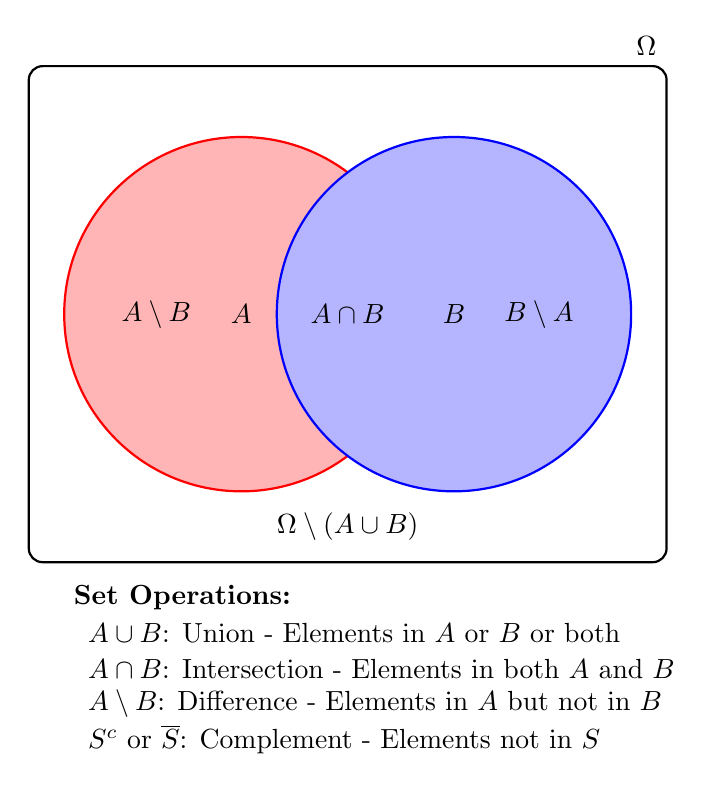
\begin{tikzpicture}[scale=0.9]
    % Define colors with opacity
    \definecolor{setA}{RGB}{255, 150, 150}
    \definecolor{setB}{RGB}{150, 150, 255}
    \definecolor{intersection}{RGB}{200, 150, 200}
    
    % Draw universal set as a rectangle
    \draw[rounded corners=5pt, thick] (-4.5,-3.5) rectangle (4.5,3.5) node[above left] {$\Omega$};
    
    % Draw sets A and B as circles
    \filldraw[fill=setA!70, draw=red, thick] (-1.5,0) circle (2.5) node {$A$};
    \filldraw[fill=setB!70, draw=blue, thick] (1.5,0) circle (2.5) node {$B$};
    
    % Label regions
    \node at (-2.7,0) {$A \setminus B$};
    \node at (2.7,0) {$B \setminus A$};
    \node at (0,0) {$A \cap B$};
    \node at (0,-3) {$\Omega \setminus (A \cup B)$};
    
    % Legend
    \begin{scope}[shift={(0,-5)}]
        \node[anchor=west] at (-4,1) {\textbf{Set Operations:}};
        \node[anchor=west] at (-3.8,0.5) {$A \cup B$: Union - Elements in $A$ or $B$ or both};
        \node[anchor=west] at (-3.8,0) {$A \cap B$: Intersection - Elements in both $A$ and $B$};
        \node[anchor=west] at (-3.8,-0.5) {$A \setminus B$: Difference - Elements in $A$ but not in $B$};
        \node[anchor=west] at (-3.8,-1) {$S^c$ or $\overline{S}$: Complement - Elements not in $S$};
    \end{scope}
\end{tikzpicture}
\caption{Venn diagram illustrating basic set operations}
\label{fig:venn_diagram}
\end{figure}

\begin{figure}[h]
\centering
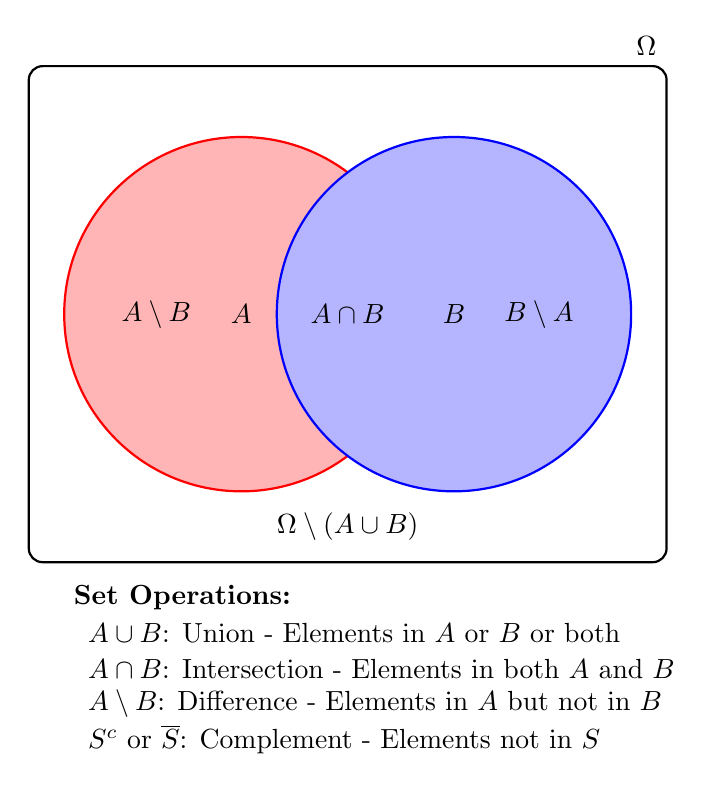
\begin{tikzpicture}[scale=0.9]
    % Define colors with opacity
    \definecolor{setA}{RGB}{255, 150, 150}
    \definecolor{setB}{RGB}{150, 150, 255}
    \definecolor{intersection}{RGB}{200, 150, 200}
    
    % Draw universal set as a rectangle
    \draw[rounded corners=5pt, thick] (-4.5,-3.5) rectangle (4.5,3.5) node[above left] {$\Omega$};
    
    % Draw sets A and B as circles
    \filldraw[fill=setA!70, draw=red, thick] (-1.5,0) circle (2.5) node {$A$};
    \filldraw[fill=setB!70, draw=blue, thick] (1.5,0) circle (2.5) node {$B$};
    
    % Label regions
    \node at (-2.7,0) {$A \setminus B$};
    \node at (2.7,0) {$B \setminus A$};
    \node at (0,0) {$A \cap B$};
    \node at (0,-3) {$\Omega \setminus (A \cup B)$};
    
    % Legend
    \begin{scope}[shift={(0,-5)}]
        \node[anchor=west] at (-4,1) {\textbf{Set Operations:}};
        \node[anchor=west] at (-3.8,0.5) {$A \cup B$: Union - Elements in $A$ or $B$ or both};
        \node[anchor=west] at (-3.8,0) {$A \cap B$: Intersection - Elements in both $A$ and $B$};
        \node[anchor=west] at (-3.8,-0.5) {$A \setminus B$: Difference - Elements in $A$ but not in $B$};
        \node[anchor=west] at (-3.8,-1) {$S^c$ or $\overline{S}$: Complement - Elements not in $S$};
    \end{scope}
\end{tikzpicture}
\caption{Venn diagram illustrating basic set operations}
\label{fig:venn_diagram}
\end{figure}

\begin{figure}[h]
\centering
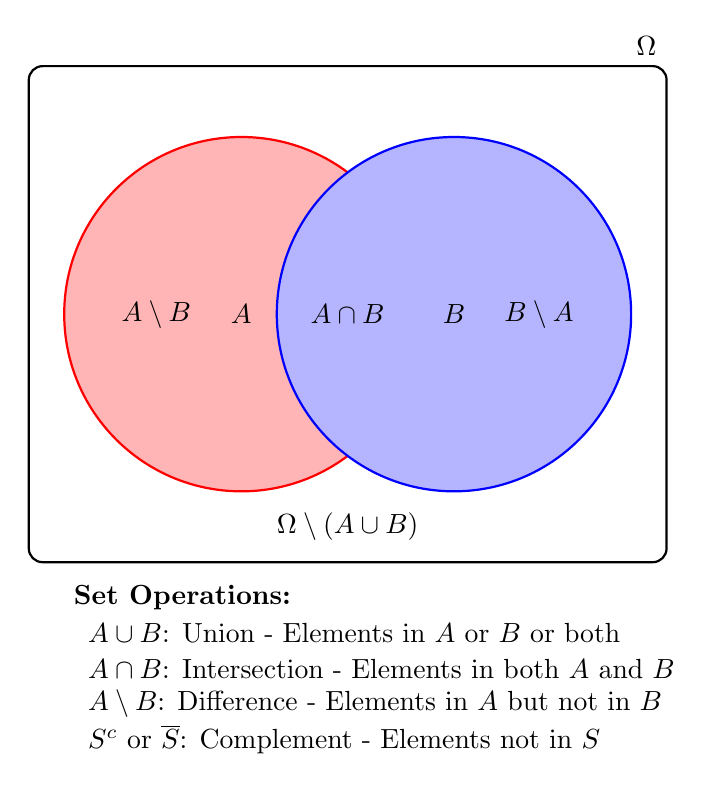
\begin{tikzpicture}[scale=0.9]
    % Define colors with opacity
    \definecolor{setA}{RGB}{255, 150, 150}
    \definecolor{setB}{RGB}{150, 150, 255}
    \definecolor{intersection}{RGB}{200, 150, 200}
    
    % Draw universal set as a rectangle
    \draw[rounded corners=5pt, thick] (-4.5,-3.5) rectangle (4.5,3.5) node[above left] {$\Omega$};
    
    % Draw sets A and B as circles
    \filldraw[fill=setA!70, draw=red, thick] (-1.5,0) circle (2.5) node {$A$};
    \filldraw[fill=setB!70, draw=blue, thick] (1.5,0) circle (2.5) node {$B$};
    
    % Label regions
    \node at (-2.7,0) {$A \setminus B$};
    \node at (2.7,0) {$B \setminus A$};
    \node at (0,0) {$A \cap B$};
    \node at (0,-3) {$\Omega \setminus (A \cup B)$};
    
    % Legend
    \begin{scope}[shift={(0,-5)}]
        \node[anchor=west] at (-4,1) {\textbf{Set Operations:}};
        \node[anchor=west] at (-3.8,0.5) {$A \cup B$: Union - Elements in $A$ or $B$ or both};
        \node[anchor=west] at (-3.8,0) {$A \cap B$: Intersection - Elements in both $A$ and $B$};
        \node[anchor=west] at (-3.8,-0.5) {$A \setminus B$: Difference - Elements in $A$ but not in $B$};
        \node[anchor=west] at (-3.8,-1) {$S^c$ or $\overline{S}$: Complement - Elements not in $S$};
    \end{scope}
\end{tikzpicture}
\caption{Venn diagram illustrating basic set operations}
\label{fig:venn_diagram}
\end{figure}

\begin{figure}[h]
\centering
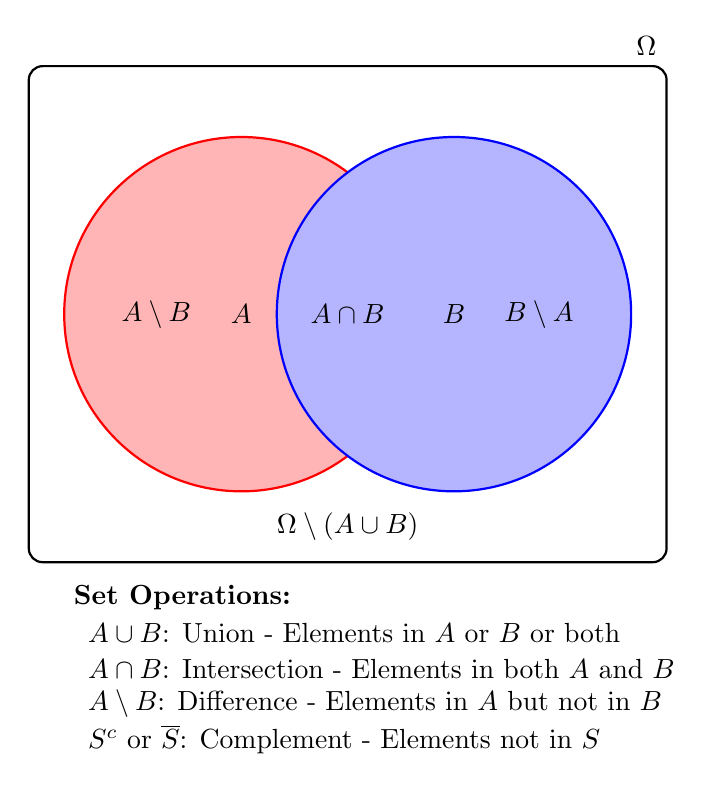
\begin{tikzpicture}[scale=0.9]
    % Define colors with opacity
    \definecolor{setA}{RGB}{255, 150, 150}
    \definecolor{setB}{RGB}{150, 150, 255}
    \definecolor{intersection}{RGB}{200, 150, 200}
    
    % Draw universal set as a rectangle
    \draw[rounded corners=5pt, thick] (-4.5,-3.5) rectangle (4.5,3.5) node[above left] {$\Omega$};
    
    % Draw sets A and B as circles
    \filldraw[fill=setA!70, draw=red, thick] (-1.5,0) circle (2.5) node {$A$};
    \filldraw[fill=setB!70, draw=blue, thick] (1.5,0) circle (2.5) node {$B$};
    
    % Label regions
    \node at (-2.7,0) {$A \setminus B$};
    \node at (2.7,0) {$B \setminus A$};
    \node at (0,0) {$A \cap B$};
    \node at (0,-3) {$\Omega \setminus (A \cup B)$};
    
    % Legend
    \begin{scope}[shift={(0,-5)}]
        \node[anchor=west] at (-4,1) {\textbf{Set Operations:}};
        \node[anchor=west] at (-3.8,0.5) {$A \cup B$: Union - Elements in $A$ or $B$ or both};
        \node[anchor=west] at (-3.8,0) {$A \cap B$: Intersection - Elements in both $A$ and $B$};
        \node[anchor=west] at (-3.8,-0.5) {$A \setminus B$: Difference - Elements in $A$ but not in $B$};
        \node[anchor=west] at (-3.8,-1) {$S^c$ or $\overline{S}$: Complement - Elements not in $S$};
    \end{scope}
\end{tikzpicture}
\caption{Venn diagram illustrating basic set operations}
\label{fig:venn_diagram}
\end{figure}